%
% File acl2016.tex
%
%% Based on the style files for ACL-2015, with some improvements
%%  taken from the NAACL-2016 style
%% Based on the style files for ACL-2014, which were, in turn,
%% Based on the style files for ACL-2013, which were, in turn,
%% Based on the style files for ACL-2012, which were, in turn,
%% based on the style files for ACL-2011, which were, in turn,
%% based on the style files for ACL-2010, which were, in turn,
%% based on the style files for ACL-IJCNLP-2009, which were, in turn,
%% based on the style files for EACL-2009 and IJCNLP-2008...

%% Based on the style files for EACL 2006 by
%%e.agirre@ehu.es or Sergi.Balari@uab.es
%% and that of ACL 08 by Joakim Nivre and Noah Smith

\documentclass[11pt]{article}
\usepackage{acl2016}
\usepackage{times}
\usepackage{url}
\usepackage{latexsym,graphicx,listings,hyperref}

\aclfinalcopy % Uncomment this line for the final submission
%\def\aclpaperid{***} %  Enter the acl Paper ID here

%\setlength\titlebox{5cm}
% You can expand the titlebox if you need extra space
% to show all the authors. Please do not make the titlebox
% smaller than 5cm (the original size); we will check this
% in the camera-ready version and ask you to change it back.

\newcommand\BibTeX{B{\sc ib}\TeX}
\lstset{basicstyle=\ttfamily\footnotesize,breaklines=true}

\title{A Dependency-Parser-Based Approach to Converting Natural Language English Sentences to Karel J\ Robot Code}

\author{
    % First Author \\
    % Affiliation / Address line 1 \\
    % Affiliation / Address line 2 \\
    % Affiliation / Address line 3 \\
    % {\tt email@domain} \\\And
    % Second Author \\
    % Affiliation / Address line 1 \\
    % Affiliation / Address line 2 \\
    % Affiliation / Address line 3 \\
    % {\tt email@domain} \\}
    Christopher Fu \\
    \texttt{christopher.fu@yale.edu} \\}
\date{}

\begin{document}
\maketitle
\begin{abstract}
  This document contains the instructions for preparing a camera-ready
  manuscript for the proceedings of ACL-2016. The document itself
  conforms to its own specifications, and is therefore an example of
  what your manuscript should look like. These instructions should be
  used for both papers submitted for review and for final versions of
  accepted papers.  Authors are asked to conform to all the directions
  reported in this document.
\end{abstract}

\section{Introduction}
Programming students often find that when they are first learning how to to program, accurately
translating what they want their program to do into actual code is harder than expected. Newell and
Card~\shortcite{Newell:1985aa} suggest that one factor contributing to this difficulty is that most
popular programming languages are not particularly designed with human-computer interaction issues
in mind. Some programming languages more easily lend themselves to a natural translation between
programmer intent and actual code, a concept that Green and Petre~\shortcite{Green:1996aa} term
\emph{closeness of mapping}.

Consider the following example based on one that Green and Petre give: we wish to sum up a sequence
of $N$ integers. In C, we could write a program like the one shown in Figure~\ref{fig:c-prog}.
Though writing such a program is second-nature for an experienced programmer, there is a large
amount of implicit knowledge contained in such a program that must be remembered by a novice
programmer. For example, we must recall the syntax of a variable declaration and a \texttt{for}
loop, and we must remember which lines must be terminated with a semicolon which lines do not. We
must also recall that arrays are 0-indexed, and the indexing variable \texttt{i} must run from 0 to
$N - 1$. Even experienced programmers may inadvertently commit a so-called ``off-by-one error''
from time to time. On the other hand, in Python, we could write a program shown in Figure
~\ref{fig:python-prog}. The Python program does away with much of the C program's syntactical
clutter---there are no curly braces to delimit a block and no \texttt{for} loop to begin with---
and the (intuitively-named) function \texttt{sum()} performs the summing action.  The Python
program more closely maps the programmer's intent and the actual code required to realize his
intent.

\begin{figure}[ht]
\begin{lstlisting}[language=C]
int s = 0;
for (int i = 0; i < N; i++) {
    s += arr[i];
}
\end{lstlisting}
\label{fig:c-prog}
\caption{C program calculating the sum of $N$ integers in \texttt{arr}.}
\end{figure}

\begin{figure}[ht]
\begin{lstlisting}[language=python]
s = sum(arr)
\end{lstlisting}
\label{fig:python-prog}
\caption{Python program calculating the sum of $N$ integers in \texttt{arr}.}
\end{figure}

In addition to using a more natural programming language, students also often work with a
restricted subset of a programming language to prevent all of the complexities of the language from
overwhelming them. In high school and university introductory-level programming courses, Karel J
Robot is a popular library that is used to teach students objected-oriented Java
programming~\cite{Bergin:2013aa}. In the Karel universe, there are three types of entities---
robots, beepers, and walls. Robots can move around on a 2D grid and pick up or drop beepers at grid
coordinates. Walls impede the movement of robots, and robots that attempt to move through a wall
blocking their path will shut down. Robots also have the ability to check if they occupy the same
grid coordinate, if they are in front of a wall, or if they are facing in one of the four cardinal
directions. Figure~\ref{fig:karel-ex} shows an example of a Karel world with a robot facing south
and two beepers. A description of the Karel J Robot API can be found at
\url{http://www.cs.gordon.edu/courses/cs112/KJRdocs/index.html}.

\begin{figure}[ht]
\centering
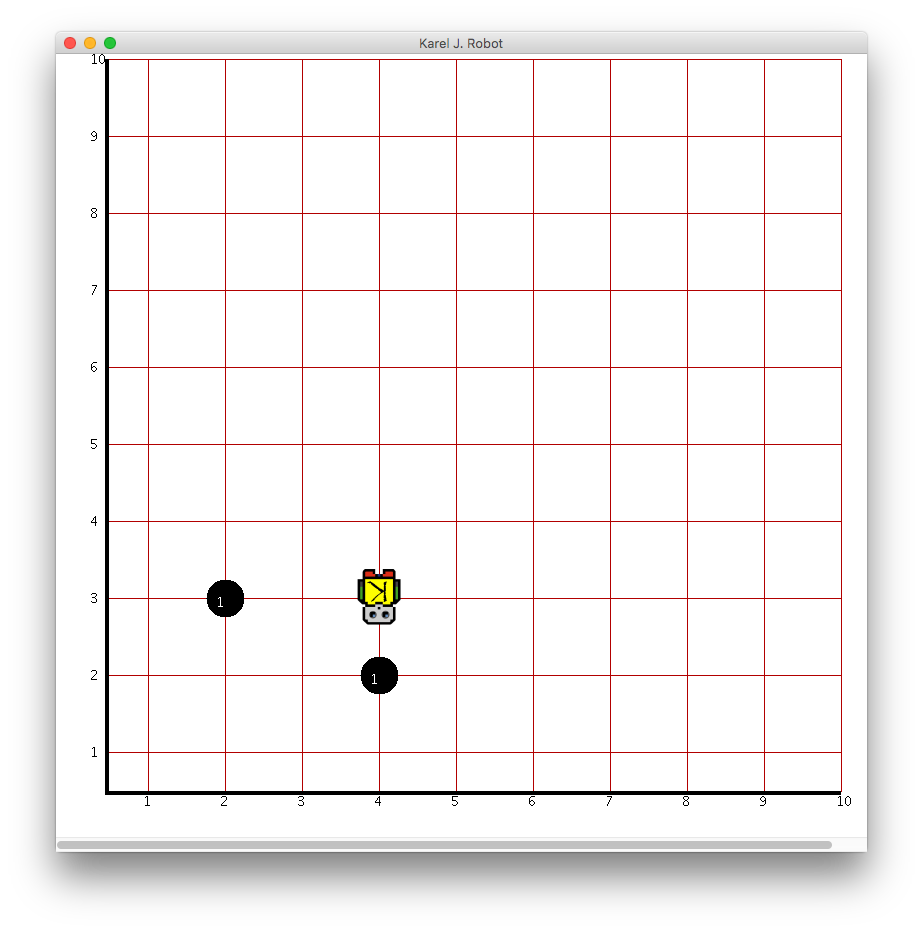
\includegraphics[width=0.5\textwidth]{karel-ex.png}
\caption{An example Karel world with a robot facing south and two beepers.}
\label{fig:karel-ex}
\end{figure}

We aim to construct a parser and code generator that converts English language sentences into Karel
J Robot Java source code. Such an application may be helpful to novice programmers who have an
approach to solving a problem that they can articulate naturally in English but do not know how
exactly to convert their approach into actual code.

\section{Existing Work}
This project is heavily inspired by Metafor, an application written by Hugo Liu and Henry Lieberman
at the MIT Media Lab~\shortcite{Liu:2005aa}. Metafor presents an interface to the user to type a
story in English describing a scenario. As the user adds more details to his story, Metafor
develops a side-by-side ``visualization'' of the person's narrative in ``pseudo-Python''
\emph{scaffolding code}, which may not necessarily be directly executable but roughly describes the
user's intent behind the narrative. Metafor is integrated with a large knowledge base of common
sense knowledge, a programmatic interpreter that identifies special constructs and objects for
which there exists some common-sense-type information (e.g., colors and flavors), and a knowledge
representation of the code model that dynamically updates itself as new information from the user
is incorporated.

\section{Approach}
In the time available, we were only able to implement and test a simple approach, which consists of
two phases: a parsing phase to convert English language sentences into a list of action statements
that represent the actions a Karel robot should take to satisfy the intent conveyed by the
sentence, and a code generation phase to generate Java code from the output of the parsing phase.
In the parsing phase, we first perform a search of the sentence to be parsed for words we were
interested in. Such words include verbs that indicate a Karel robot action of some sort (e.g.,
``move'' and ``turn''), numbers and directions that modify actions in some way (e.g. ``two'' and
``north'' in the sentence ``Move two spaces north.''), and verbs that indicate a type of
conditional statement (e.g., ``facing'' in ``if Karel is facing north''). \texttt{while} and
\texttt{for} loops are not supported at this time. These words are then grouped together using
information from the Stanford CoreNLP dependency parser~\cite{Manning:2014aa}. These groupings are
then converted into discrete action or conditional statements, which are one-to-one mappings to
lines of Karel Java code, based on what types of words are in each grouping. In the code generation
phase, we convert the actions and conditionals into Java code and inject the into a template file
that contains some boilerplate code that handles world initialization and visualization. This final
Java file output can be provided to the student to aid them in visualizing how their English
language Karel commands can be expressed in Karel Java code. The Java source can also be compiled
and run in a Karel simulator supplied in \texttt{KarelJRobot.jar}

\begin{figure}[ht]
\centering
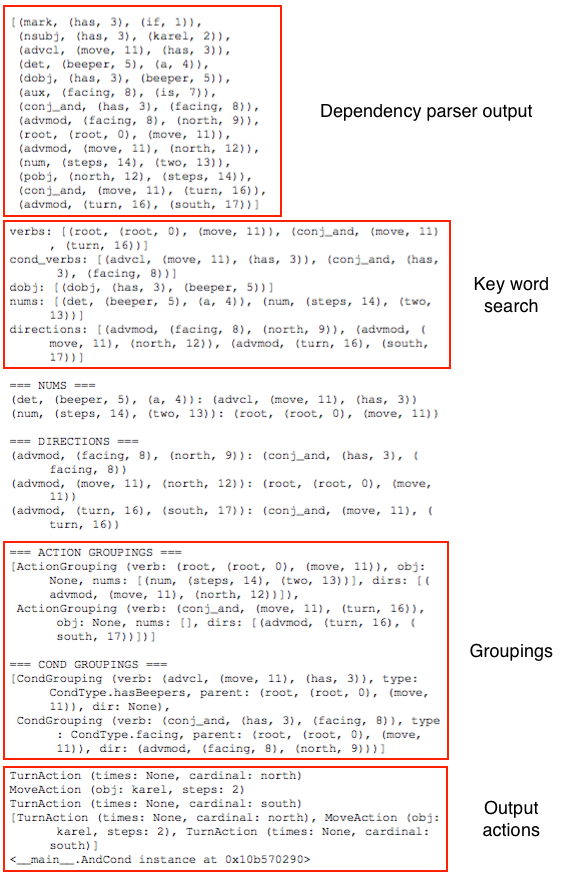
\includegraphics[width=0.5\textwidth]{parse-output.png}
\caption{Parser output for the sentence ``If Karel has a beeper and is facing north, move north two
steps and turn south.''}
\label{fig:parse-output}
\end{figure}

\begin{figure}[ht]
\begin{lstlisting}[language=java]
if (karel.anyBeepersInBeeperBag() && karel.facingNorth()) {
    while (!karel.facingNorth()) {
        karel.turnLeft();
    }
    karel.move(2);
    while (!karel.facingSouth()) {
        karel.turnLeft();
    }
}
\end{lstlisting}
\label{fig:injected-code}
\caption{The parser output in Figure~\ref{fig:parse-output} is converted into Java code in the code
generation phase, which is injected into a Java source file that can be compiled into a Java class
file.}
\end{figure}

To test the accuracy of our parser, we used a simple scheme in which we hand-wrote XX test cases.
Each test case consists of a text file containing an English sentence, a start Karel world
(\texttt{.kwld}) file, and an expected end Karel world file. Each start and end Karel world file
contains a full text description of the state of the world at the start and end of each test
case---the size of the world; the positions and numbers of beepers at grid coordinates; the
position, orientation, and number of beepers held by the robot; and the position and orientation of
walls between grid coordinates. Assuming that the input sentence could be parsed and the generated Java source could be compiled, we run the compiled Java program in the Java Karel simulator
provided by~\newcite{Bergin:2013aa} and obtain the final world state and compare it to the expected
final world state. We scored our parser's accuracy on an all-or-nothing scale: if the test and
expected final world states match exactly in beeper number and position and robot position,
orientation, and number of beepers held, the test case scores one point; otherwise, it scores zero
points.

\section{Results}

% include your own bib file like this:
%\bibliographystyle{acl}
%\bibliography{acl2016}
\bibliography{report}
\bibliographystyle{acl2016}

\appendix

\section{Supplemental Material}
\label{sec:supplemental}
ACL 2016 also encourages the submission of supplementary material
to report preprocessing decisions, model parameters, and other details
necessary for the replication of the experiments reported in the
paper. Seemingly small preprocessing decisions can sometimes make
a large difference in performance, so it is crucial to record such
decisions to precisely characterize state-of-the-art methods.

Nonetheless, supplementary material should be supplementary (rather
than central) to the paper. It may include explanations or details
of proofs or deriations that do not fit into the paper, lists of
features or feature tempates, sample inputs and outputs for a system,
pseudo-code or source code, and data. (Source code and data should
be separate uploads, rather than part of the paper).

The paper should not rely on the supplementary material: while the paper
may refer to and cite the supplementary material will be available to the
reviewers, they will not be asked to review the
supplementary material.

Appendices (i.e. supplementary material in the form of proofs, tables,
or pseudo-code) should come after the references, as shown here. Use
\verb|\appendix| before any appendix section to switch the section
numbering over to letters.

\section{Multiple Appendices}
\dots can be gotten by using more than one section. We hope you won't
need that.

\end{document}
